\documentclass[assd_tpf_lineasinvest.tex]{subfiles}

\begin{document}
\section{Filtros basados en EDPs}
En la década del 70, un inconveniente que se tuvo que enfrentar en el procesamiento de imágenes fue que al aplicar transformaciones sobre las imágenes, la transformación deterioraba los bordes de la misma. Por ejemplo, si tenemos un gato y un perro en una imagen, queremos hacer difusión sobre las partes dentro de los mismos y dejar los bordes que los separan intactos. Para poder solventar este inconveniente se propusieron distintos métodos que utilizaban ecuaciones diferenciales parciales, las cuales permiten diferir qué zonas se va a procesar.
El primer modelo presentado que apuntaba a esta solución fue hecho por Witkin en 1983, el cual consistía en convolucionar la imagen con un filtro gaussiano.

\[ I(x,y,t) = I(x,y,0)*G(x,y;\sigma_t)  \]

Donde $I(x,y,0)$ es la imagen original.


En 1984, Koenderink observó que las imágenes obtenidas podrían ser vistas como la solución a la ecuación de la difusión del calor:

\[ \frac{\partial I(x,y,t)}{\partial t} = \Delta I(x,y,t)= \frac{\partial^2I(x,y,t)}{\partial^2x} + \frac{\partial^2I(x,y,t)}{\partial^2y}   \]

Donde nuevamente la condición inicial es $I(x,y,0)$, la imagen original.
\subsection{¿Por qué la ecuación del calor?}
Los procesos de difusión están altamente relacionados con las leyes de conservación, es decir en sistemas donde hay una cierta concentración o temperatura I, sucede que hay un flujo de las regiones de mayor concentración a uno de menor concentración hasta que el sistema alcanza el equilibrio.
\subsection{¿Qué problemas conlleva utilizar el Laplaciano?}
Como el operador laplaciano es un operador isótropo, la ecuación del calor no tiene direcciones preferentes, lo cual hace que sea igualmente aplicada en todas las direcciones del plano. Este tipo de flujo es llamado  \textit{difusión isotrópica}.

\begin{figure}[H]
\begin{centering}
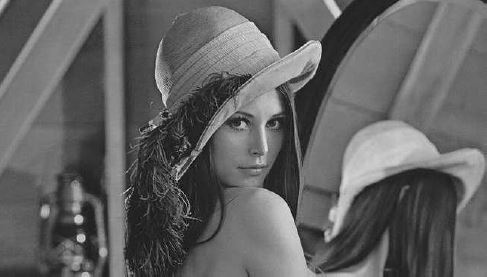
\includegraphics[scale=0.5]{original.JPG}
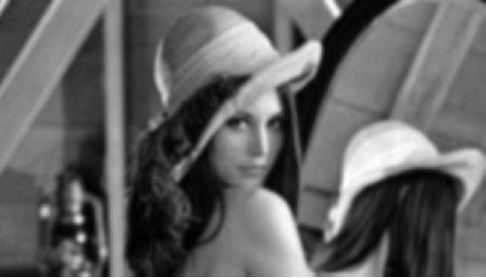
\includegraphics[scale=0.5]{confiltro.JPG}
\par\end{centering}
\caption{En la izquierda se encuentra la foto original y en la derecha se puede ver el resultado de haber aplicado difusión isotrópica}
\label{fig:ComparacionDifIso}
\end{figure}
En la figura \ref{fig:ComparacionDifIso} se puede ver que la imagen se encuentra totalmente destruida.

\section{Difusión anisotrópica } 
Hummel en 1986 establece que para obtener un buen resultado en el realce de la imagen, el flujo del filtro con el que se implemente satisfaga el principio del máximo. 
Desde ese entonces, aparecieron propuestas tales como PDE no lineales en las que no difunda el flujo uniformemente a pesar de no cumplir con el principio del máximo. Estos filtros son llamados de difusión anisotrópica. 
Pietro Perona y Jitendra Malik fueron quienes en 1990 presentaron un suavizado miltiescala preservando bordes basados en 3 criterios:

\begin{itemize}
  \item Causalidad: Disminuir la resolución de la imagen no puede dar nuevos detalles.
  \item Localización inmediata: los límites de las regiones deben ser distinguibles y coincidir con los de la imagen original
  \item Suavizado según zona: suavizado debe ser mayor dentro de una región que en sus fronteras
\end{itemize}

Este modelo se basa en la segunda ley de Fick, con un coeficiente de conductividad variable c(x,y,t) que controla la difusión en $\Omega$

  \[
    \left\{
                \begin{array}{ll}
                  I_t = div(c(x,y,t)\cdot \nabla I) \\
                  I(x,y,0) = I_0(x,y)\\
                \end{array}
              \right.
  \]
Donde 

$div(c(x,y,t) \nabla I) = \nabla \cdot (c(x,y,t) \nabla I) =c\Delta I + \nabla c \cdot \nabla I$
\\


Lo deseable según Perona y Malik es que el coeficiente de difusión c dependa de la norma del gradiente en cada punto. De esta forma, los gradientes con normas pequeñas (zonas homogéneas) tengan coeficiente alto ( filtrado fuerte, por ende suavizado). Mientras que para una norma grande, el coeficiente sea pequeño con tal de que no se deterioren los bordes, es decir que el proceso de difusión sea lento.

Asumiendo $s= |\nabla I|$ , dos propuestas que surgieron para c fueron:

Función de Lorentz:

\[
  c(s^2) = \frac{1}{1+ \frac{s^2}{K^2}}
\]

Función de Leclerc:

\[
  c(s^2) = e^{-\frac{s^2}{2K^2}}
\]

Donde K es una constante que se elige experimentalmente para controlar al sensibilidad ante los bordes.

 El filtro que se aplica es isotrópico localmente pero la diferencia es que al adaptarse de distinta forma a regiones homogéneas y no homogéneas, adopta el nombre de anisotrópico (aunque técnicamente es difusión no lineal). 

\end{document}
